\chapter{Métricas}
%\subsection{Métricas}

¿Para qué medir? Si no medimos no podemos adaptarnos bajo un marco empírico como propone Scrum. Medimos en forma transparente, en procesos de inspección y adaptación. Las métricas ayudan al equipo a evaluar su propio desempeño en el proceso de trabajo, para poder hacer cambios basados en hechos. También es un soporte a la gestión de proyecto/producto para poder medir el progreso en cuanto a impacto de negocio (no a seguir un plan), tomar decisiones de negocio, revisar la actividad de generación de valor y el desempeño\footnote{Las métricas se pueden usar para medir desempeño, pero no se deben utilizar en forma punitiva ni tampoco en sistemas de evaluación de desempeño de empleados.} del equipo en cuanto a grado de madurez o evolución. Además hay indicadores de calidad de producto que nos pueden señalar aspectos claves de prestancia y salud de un producto. Se puede ver a las métricas como parte del monitoreo de salud del equipo, sistema de trabajo, producto y negocio; y parte del sistema de estabilización de la empresa y del sistema de mejora continua y aprendizaje.

En síntesis, se pueden categorizar a las métricas en cuatro aspectos: trabajo en equipo (team), proceso de trabajo (process), calidad de producto (quality) e impacto de negocio (Impact) [ver fig. \ref{fig:Metrics_KPIs}].

\begin{figure}[h]
  \centering
  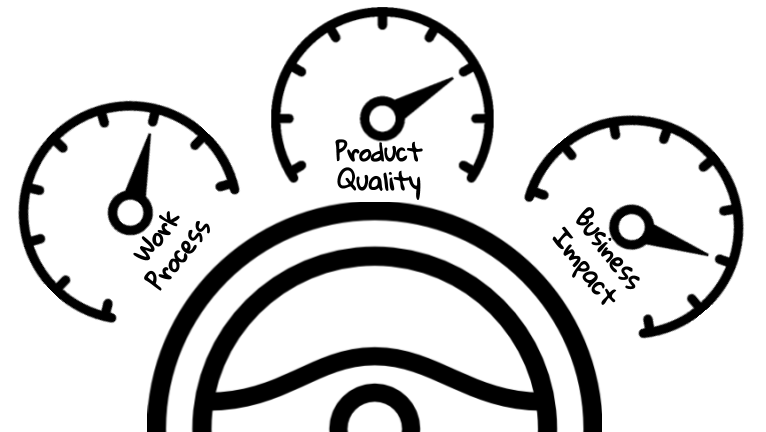
\includegraphics[width=0.85\textwidth]{Metrics_KPIs}
  \caption{Modelo de 4 categoría de métricas o KPIs.}
  \centering
  \label{fig:Metrics_KPIs} %\ref{fig:Metrics_KPIs}
\end{figure}
\FloatBarrier % Command to control the position of floating images. With its, I can get the figures not to be pushed to the end of the document.
% El comando FloatBarrier es usado aqui para que la imagen se clave en este lugar y que no sea acarreada al final del documento.

\subsection{Métricas de equipo}

El trabajo colaborativo es uno de los cuatro aspectos claves de la agilidad. Por tal motivo podemos medirlo de alguna manera simple para ayudar en la mejora contínua del equipo. A continuación puedo mostrar algunas sugerencias.

\begin{enumerate}

\item {\textbf{Team Happiness:} Un estudio de Harvard muestra que la felicidad aumenta la producción de cualquier tipo de trabajo, pues "la gente feliz es 12 \% más productiva"\footnote{\cite{U-K-University-2014}}. Además, un principio de la agilidad es desarrollar en torno a individuos motivados. En base a esto podemos intentar medir la felicidad Sprint a Sprint\footnote{\cite{Jeff-2014}}. 

La felicidad del equipo es un indicativo de la salud del equipo en relación a su capacidad de entrega de valor. Para medir la felicidad del equipo podemos hacer encuestas o responder las siguientes preguntas:

  \begin{enumerate}
  \item {¿Cómo me siento acerca de mi trabajo? Se puede usar una escala de 1 a 5 (ver figura \ref{fig:HappinessMetric}). 
  
  \begin{figure}[h]
  \centering
  
\includegraphics[width=0.40\textwidth]{HappinessMetric}
  \caption{Medida de satisfacción}
  \centering
  \label{fig:HappinessMetric} %\ref{fig:HappinessMetric}
  \end{figure}
  \FloatBarrier

  Otra escala para medir felicidad puede ser de siete puntos. Por ejemplo a la pregunta... ¿Cómo calificaría su felicidad en este momento? Se puede responder con 1 que es totalmente triste, 2 es muy triste , 3 es triste, 4 es ni feliz ni triste, 5 es bastante feliz, 6 es muy feliz y 7 es completamente feliz\footnote{\cite{U-K-University-2014}}.
  }
  
  \item {¿Qué va a hacer que me sienta mejor?}
  \end{enumerate}

Cuando tenemos la información de cada miembro del equipo, el equipo puede hacer una lluvia de ideas de cómo hacer para mejorar y aumentar la felicidad en el siguiente Sprint y darle curso y seguimiento a las acciones propuestas.

}

\item {\textbf{Team Morale:} Indicador moral de equipo dice cómo está la moral en tu equipo. La moral del equipo es una medida más estable y confiable que la felicidad del equipo \footnote{Agile Teams: Don't use happiness metrics, measure Team Morale. Agilistic, Christiaan Verwijs, 2014.}. Esta métrica mide el orgullo, entusiasmo, energía, resiliencia, disposición para ayudarse mutuamente y motivación por el significado y propósito. Se puede medir mediante encuestas periódicas. Un cuestionario simple y práctico puede ser el siguiente (Las preguntas individuales se califican en una escala de 1 a 7 o de 1 a 5):
  \begin{enumerate}
  \item {¿Me siento bien (siento que encajo) y me siento fortalecido en mi equipo?}
  \item {¿Estoy orgulloso del trabajo que hago para mi equipo?}
  \item {¿Estoy entusiasmado con el trabajo que hago para mi equipo?}
  \item {¿Encuentro el trabajo que hago para mi equipo de significado y con propósito?}
  \end{enumerate}
}

\item {\textbf{Team Stability:} Se considera que se logra buena colaboración con equipos estables. Por ese motivo, bajo el marco ágil, se prioriza a los equipos estables por sobre los proyectos\footnote{The Disciplined Agile (DA) Framework}. Es decir que se recomienda mantener a los equipos estables y evitar mezclar personas entre equipos o desarmar equipos para asignar a otros proyectos (la rotación). Los equipos estables tienden a conocer mejor su capacidad, lo que permite cierta capacidad de predicción y mayor sinergia. Los miembros del equipo deben dedicarse a un solo equipo siempre que sea posible. Pero esto no siempre se logra por la rotación laboral o necesidades de la empresa. Por eso es útil medir el aspecto de “Team Stability” o  de rotación. Pues hay que mantener una rotación baja saludable.
}

\item {\textbf{Team Skill Balance:} Si existe un desbalance de conocimientos y de esfuerzo en el equipo puede provocar la fatiga de algunos integrantes, problemas por eslabones débiles (en contingencias, entrevistas, solución de problemas, etc.), dependencias sobre alguna persona o desavenencias por percepción de inequidad de esfuerzos. Un indicador de balance de competencias del equipo (Team Skill Balance Average) podría ayudar a que el equipo sea capaz de trabajar como una unidad integrada. Cada integrante debe ser un poco más multifuncional, colaborando en tareas o actividades que no son su fuerte o especialidad. 
}

\end{enumerate}

\subsection{Métricas del proceso de trabajo}

La entrega de valor fluida y continua es otro de los cuatro aspectos claves de la agilidad. Para mejorar este flujo de valor se busca, entre otras cosas, un flujo estable, sostenible y en un proceso de trabajo limpio (sin impedimentos ni desperdicios). En este sentido hay muchos indicadores clave del proceso de trabajo, de rendimiento, internos del equipo, que nos pueden ser de utilidad para monitorear el proceso de desarrollo y que nos permita la inspección y adaptación constante, como por ejemplo los siguientes\footnote{Scott y Jeff \cite{Scott-Jeff-2013} y la  Scrumalliance en un artículo llamado "Velocity, How to Calculate and Use Velocity to Help Your Team and Your Projects", por Catia Oliveira (6 February 2014).}:

\begin{enumerate}

\item {\textbf{Velocity:} La 'velocidad'\footnote{"Sum of original estimates of all accepted work" \cite{Scott-Jeff-2013}.} es el número de unidades de trabajo o puntos de historia SP estimados y aceptados por un equipo en una iteración Sprint. En otras palabras, es el conjunto de puntos de historia totales conseguidos (aceptados) por el equipo al final de cada Sprint\footnote{\cite{Jipson-Thomas-2015}}. Aquí hay que tener en cuenta que el Story Points o SP es una unidad de medida que indica una cantidad de alcance o trabajo que puede ser entregado o tamaño de producto estimado para entregar. Representa la complejidad o esfuerzo necesario para terminar las tareas de una historia \footnote{\cite{Jipson-Thomas-2015}}. El SP sirve como estimación de la complejidad en forma relativa y sumativa que hacen los desarrolladores. También hay que tener en cuenta que es una unidad subjetiva que depende de qué equipo hace la estimación de medida.} 

Esta definición es la clásica y es algo genérica. Hay tres formas más específicas de interpretar y medir la velocidad:

  \begin{enumerate}

  \item{\textbf{Velocidad de trabajo:} cuando la velocidad muestra la cantidad de trabajo o funcionalidad que un equipo entrega (aceptada) en un sprint\footnote{"Velocidad en la que el equipo pueda completar el trabajo en un Sprint, número de funcionalidades entregadas en un sólo Sprint o Número de Story Points hecho en un determinado Sprint" \cite{SBOK-2013}}, incluyendo las de valor indirecto. En este sentido, las historias de usuarios completadas (tomadas del backlog técnico) que tienen valor indirecto para el cliente, las correcciones de errores, deuda técnica, migraciones y refactorizaciones sí cuentan en la velocidad. En este caso, la velocidad del equipo da pocas indicaciones sobre el verdadero valor de negocio entregado y más sobre la capacidad que puede producir. Pues la velocidad, en este sentido, no suele tener relación directa con el valor de negocio entregado. Como no se suele aclarar bien la definición de velocidad se suele entender que se trata de esta perspectiva pero, sin embargo, en Scrum clásico se sobreentiende que los equipos deben entregar valor de punta a punta, por lo que la velocidad debería estar ligada al valor como la siguiente definición.
  }

  \item{\textbf{Velocity en nueva funcionalidad:} cuando la velocidad muestra solo la cantidad de funcionalidad de valor para el negocio que un equipo entrega (aceptada) en un sprint. En este sentido, las historias de usuarios que no tienen ningún valor para el cliente o incompletas, las correcciones de errores y las refactorizaciones no cuentan en la velocidad\footnote{\cite{David-Koontz-2014}}. En este caso, la velocidad del equipo da un indicio sobre el valor de negocio entregado por el equipo. En Scrum original o clásico se sobre-entiende que las historias son las que aportan valor, por tal motivo a veces no se aclara explícitamente esto.
  }
  
  \item{\textbf{Value Velocity:} es una forma interesante para medir la productividad (sugerida por James Shore\footnote{\cite{James-Shore-2015}}) similar a la velocidad tradicional o velocidad de trabajo, excepto que se basa en estimaciones de valor de negocio (Business Value Point) hechas por el PO antes de la planeación.
  }
  
  \end{enumerate}

\item {\textbf{Average Velocity:} De la velocity de cada Sprint se calcula la velocidad promedio o "Average Velocity" que es el número de unidades de trabajo o SP promedio estimados y aceptados por un equipo en un conjunto de iteraciones Sprint. En un equipo ágil de velocidad estable, la velocidad promedio (por ejemplo de los últimos 4 Sprints) es un indicador adelantado de la velocidad estimada para el próximo Sprint (bajo las mismas condiciones de los Sprints usados para calcularla).}

\item {\textbf{Work Capacity:} La Capacidad es la suma de todos los trabajos reportados durante el Sprint, esten terminados o no\footnote{Scott y Jeff \cite{Scott-Jeff-2013}}. La capacidad es generalmente igual o superior a la Velocity. Aunque la Capacidad puede, en raras ocasiones, caer por debajo de la velocidad. Esto se debe a que la velocidad se calcula en base a las estimaciones originales de trabajo, mientras que la capacidad se calcula en base a la suma de trabajo real reportado\footnote{Scott y Jeff \cite{Scott-Jeff-2013}}. Por lo que en el caso de que esto suceda, lo que indica es que el equipo ha sobre estimado la complejidad de los trabajos solicitados. También existen otras formas de calcular o entender la capacidad. Por ejemplo:

  \begin{enumerate}
  
  \item {\textbf{Capacidad en puntos ideales:} La capacidad puede ser una idealización basada en la velocidad promedio, o sea, los puntos de la historia que se pueden considerar gastar en la próxima carrera de velocidad.\footnote{\cite{Satish-Thatte-2013}}}

  \item {\textbf{Capacidad en horas:} La capacidad puede ser calculada en horas basados en la cantidad de miembros y la cantidad de horas efectivas de trabajo en un Sprint. Por ejemplo en un equipo de 8 miembros, con 6 horas de trabajo efectivo y un Sprint de 10 días, la capacidad en horas es igual a 480 hs (8 x 6 hs x 10).}

  \end{enumerate}

Cuando se definió el marco de trabajo, como algo mínimo de cosas para que funcione, se dejó lo más simple posible. Debido a ello, el concepto de Velocity es partes del marco de trabajo aceptada por la comunidad, pero Working capacity no lo es del todo aceptado, aunque es ampliamente usado.
}

\item {\textbf{Focus Factor:} El factor de foco revela el foco que el equipo ha tenido para entregar valor y su prestancia. El mismo es la relación entre la Velocity y la capacidad de trabajo: ( Velocity / Work Capacity ) x 100\%. La misma debe permanecer en la vecindad de 80 \% en promedio para un equipo saludable. Estos puntos de datos por debajo del 80 por ciento indican un equipo que está interrumpido o incapaz de convertir su trabajo estimado en trabajo aceptado mostrando poca previsibilidad. Cuando el valor es alto, cercano al 100, el equipo ha estado bajo la previsión de su capacidad, aunque esto no indica necesariamente que están trabajando bien. Por ejemplo, el equipo puede estar aparentando ser perfecto forzando la coincidencia.}

\item {\textbf{Targeted Value Increase (TVI+):} El TVI+ responde a cuánto cambio ha habido en la velocidad del equipo a través del tiempo desde el primer Sprint. Es la Velocity del Sprint actual dividido la Velocity Original (velocity del primer sprint): ( Current Sprint’s Velocity / Original Velocity ) x 100\%. Sirve para medir el aumento de la contribución de valor de un equipo en base a su velocidad origen Sprint a Sprint.
Por ejemplo, si el resultado es 200\% significa que el equipo ha duplicado su capacidad de resolver con éxito la complejidad requerida.
}

\item {\textbf{Effectiveness:} La efectividad de un sprint medida como historias o features entregadas (aceptadas) versus las elegidas en la planning (las que se tomaron en el sprint). También se podría medir la efectividad relacionada a si se cumplió con el objetivo del sprint.
}

%Otras: Percentage of Adopted Work, Percentage of Found Work, Accuracy of Estimation, Accuracy of Forecast, Targeted Value Increase (TVI+), Success at Scale

\item {\textbf{Delivery rate:} La tasa de entrega es un indicador que nos puede servir para ver la evolución de los tiempos de entrega. Nos puede ayudar a mejorar el continuous delivery.
}

\item {\textbf{Métricas de flujo:} Scrum no prescribe métricas, por lo que bien podrían usarse métricas de flujo en vez de las basadas en SP, tomando cosas del método kanban. Algunas de ellas son el Throughput, Lead time (Lt) y Cycle time (Ct). Siendo el Throughput la velocidad, como número medio de unidades procesadas en un tiempo determinado. El Lead time, tiempo total en que una unidad pasa por el sistema de trabajo. Y el Cycle time, tiempo real de trabajo sobre una unidad sin los tiempos de cola o espera.
}

\end{enumerate}

\subsection{Métricas de calidad de producto}

Bajo el marco ágil buscamos la excelencia técnica y en esa vía buscamos productos de calidad excelente. Pues bien, como se imaginan, tendremos que medir de algún modo la calidad de nuestro producto, ya sea calidad interna o del producto operando. Podemos citar algunos indicadores.

  \begin{enumerate}    

  \item {\textbf{Maintainability:} Hay métricas asociadas a la mantenibilidad, como lo son: test Coverage, CLOC, issues, complexity,  etcétera. 
  
    \begin{enumerate}    
    \item {\textbf{Test coverage:}
Por ejemplo la cobertura de prueba es una herramienta útil para encontrar partes no probadas de una base de código, lo cual nos ayuda a saber si se están realizando pruebas suficientes para apoyar el aseguramiento de calidad.
}
  \end{enumerate}
}

  \item {\textbf{Reliability:} La fiablilidad es una medida de qué tan robusta es una aplicación. Puede ser medida con otros KPI indirectos como defectos escapados (Escaped defects), tasa de errores (Error rate) o tiempo medio entre fallos (mean time between failures).
  
  \begin{enumerate}    
    \item {\textbf{Escaped defects:}
Un defecto escapado es un defecto que no fue encontrado por el equipo en el proceso de desarrollo y que escapó al control de calidad interno del equipo. Por lo general, esos problemas son incidentes en operaciones (OPCON), es decir que los encuentran los usuarios finales una vez que la versión de release fue publicada y puesta a su disposición. Su cálculo más simple es cantidad en un período dado (por ejemplo cantidad de OPCON por sprint). Como mencionamos antes, es una medida de fiabilidad, cuanto menos defectos más fiable.
}
  \end{enumerate}
  }


  \item {\textbf{Performance:}
Las métricas de prestancia o rendimiento de aplicación nos ayudan a detectar problemas o posibles mejoras. En el caso de aplicaciones web hay una infinidad de indicadores que se pueden usar como: “Availability”, “Uptime”, “Loading time”, “Average Application Response Time”, “Peak Response Time”, “Error Rate”, etcétera. El equipo debe elegir los necesarios para el contexto de operatividad y objetivos de negocio.
}

  \item {\textbf{Security:}
  Métricas relacionadas a seguridad como: "Dynamic analysis issues" o "Static analysis issues".
}

  \end{enumerate}

Estas métricas listadas son solo una guía para investigar otras y analizar cuáles pueden ser necesarias para algún caso particular.

\subsection{Métricas de impacto de negocio}

Siguiendo una de las claves de la agilidad, el flujo de entrega de valor continuo, es que podemos suponer que la verdadera medida de éxito en Scrum es el incremento de producto que es valioso. Pero, ¿qué es valioso y para quién? Cabe aclarar, que valor de negocio no se refieren solo a valor monetario, también puede ser de valor intangible, como el posicionamiento de una marca o el valor dado por mejorar la experiencia del usuario, siendo un beneficio para el usuario o cliente y, en consecuencia, también para la compañía. El valor es lo valioso para la compañía y para el cliente. Si estamos centrados en el cliente debemos pensar en qué es valioso para él. Pues bien, ¿cómo medir qué es valioso?
Scrum no prescribe métricas de negocio o indicadores clave de impacto de negocio, aunque es necesario usarlos para saber si realmente estamos entregando valor o generando el impacto deseado. El PO tiene el poder de tomar la decisión última de negocio y necesita datos empíricos para hacerlo. Además, en el proceso de inspección y adaptación, para construir el producto adecuado, el equipo con el PO necesitan observar indicadores de producto, orientarse, decidir y actuar, en busca de maximizar el valor. En esta vía, el PO tiene la posibilidad de usar Business Value Point para estimar valor entregado o hacer una distinción entre historias de usuario de cara a cliente o técnicas (más adelante explicado). Por otro lado, también se pueden manejar un conjunto mínimo y suficiente de indicadores de negocio. A estos indicadores, que se los suele llamar KPI's, podemos interpretarlos como "indicadores claves de impacto" del producto. Lo importante de los indicadores que elijamos es que deben estar alineados a la visión y objetivos que hayamos definido para el producto.
Algunos son los siguientes.



  \begin{description}    

  \item {\textbf{Business Value Delivered:} Valor de negocio entregado. Se pueden contabilizar los Business Value o BV entregados en cada Sprint. El VB es el valor añadido que la feature/historia aporta al negocio\footnote{\cite{Pointet-Botton-2012}}. A semejanza del SP, el Business Value Point o BVP sirve como estimación del valor de negocio en forma relativa y sumativa que hace el PO. También hay que tener en cuenta que es una unidad subjetiva que depende de qué PO o equipo de personas hace la estimación de medida.
} 
 
  \item {\textbf{Sh-SAT:} Grado de satisfacción de los Stakeholders. Se puede medir la felicidad de los Stakeholder como indicador de grado de satisfacción que indica qué tan contentos estuvieron con los resultados del Sprint y con la Review. Este relevamiento relacionado a la percepción de valor entregado se puede hacer en la misma Review.
}

  \item {\textbf{C-SAT:} Customer Satisfaction es el índice de grado de satisfacción de los usuarios o clientes. Porcentaje de usuarios que respondieron "sí" para encontrar el servicio o producto útil en la encuesta de comentarios en comparación con el número total de encuestados.
}

  \item {\textbf{NPS:} El Puntaje Neto de Promotores (Net Promoter Score) mide la lealtad general de los clientes hacia un producto o servicio (fidelización). Mide qué probabilidad hay de que el cliente recomiende la compañía y, de forma indirecta, la propensión del consumidor a seguir siéndolo y resistir irse a la competencia.
}

  \item {\textbf{TTM:}
El Time-To-Market es el tiempo que toma un nuevo producto/servicios desde que fue ideado o comenzó a ser conceptualizado, hasta que llega al mercado, disponible al cliente. El TTM es fundamental para el negocio en un entorno empresarial global altamente competitivo, ya que a un tiempo más corto ganamos una ventaja competitiva. La agilidad ayuda a entregar valor en forma temprana, por lo que este KPI debería mejorar en una empresa ágil.
}

  \item {\textbf{Revenue:} Beneficios o ingresos obtenidos. Se suele medir los ingresos en un periodo dado. Hay que tener en cuenta que esta medida puede ser multifactorial, o sea que el resultado de su aumento o disminución puede ser causado por otros agentes (como marketing). Por este motivo, tener un enfoque reduccionista basado exclusivamente en el beneficio no necesariamente se correlaciona con el valor realmente entregado.
}

  \item {\textbf{Cost Savings:} Grado de reducción de costos. Hay productos/servicios que impactan en la disminución de costos, prescindiendo de recursos, insumos o servicios que representan un costo para la organización.
}

  \item {\textbf{Completion rate:} La tasa de finalización mide el porcentaje de usuarios que finaliza con éxito o generan un resultado exitosamente. Se calcula dividiendo el número total de interacciones completadas con éxito por el número total de interacciones iniciadas. También se puede conocer como tasa de conversión ("Conversion Rate" en web site) o "Full Compliance", como el porcentaje de visitantes a un sitio web que cumplen el objetivo del sitio. 
}

  \item {\textbf{Volume of Use:} Cuantos usuarios usan nuestra aplicación.
}
  \item {\textbf{Penetration:} Cuantos usuarios, de los que ya son clientes, usan nuestra aplicación del volumen total que usan dicho servicio en relación a todos los canales. Esto marca la parte del “Volume of Use” que crece por que los usuarios dejan de usar otros canales.
}

  \item {\textbf{Digital take-up:} Tasa de adopción para el servicio digital \footnote{Performance Dashboard del gobierno de australia (dashboard.gov.au)}.
}

  \item {\textbf{Market Share:} Cuantos usuarios, de los usuarios que no son clientes, fueron captados. O sea, que cantidad de usuarios nuevos captados de la competencia o del mercado. Esto marca si el “Volume of Use” crece por captación de nuevos usuarios.
}

  \item {\textbf{Acquisition:} Nuevos usuarios que vienen de otros canales o usuarios que bajan y usan la aplicación por primera vez.
}

  \item {\textbf{Activation:} Usuario que se sienten feliz al usar la aplicación por primera vez. Que realmente están usando la aplicación y conectado con la aplicación o que firman y hacen una orden para hacerse clientes.
}

  \item {\textbf{Engagement:} grado de compromiso o incremento de órdenes o valor de cuenta por cliente.
}

  \item {\textbf{Retention:} Usuarios recurrentes o clientes que vuelven a usar la aplicación o que hacen órdenes mensualmente o tienen actividad mensual.
}

  \item {\textbf{Referral:} Usuarios felices que se lo dicen a sus amigos, es decir que recomiendan la aplicación.
}

  \item {\textbf{ROI:} El ROI (Return Over Investment) es tanto una técnica como una métrica e indica el retorno de una inversión, es decir, la cifra que evalúa el rendimiento del capital en una acción. Pues, nos permite cuantificar económicamente el beneficio. Su fórmula es: ROI = (IP - CP) / CP; Donde IP es el ingresos del proyecto o período, entendido como beneficios económicos esperados estimados, y CP es el Costo del proyecto o período como costo de desarrollo.
}

\end{description}

Cabe recalcar que pueden haber muchos otros KPI’s y que, los que elijamos, sean lo justo y necesario; y actúen como una brújula, que nos posibilite decidir si debemos continuar con el mismo rumbo o tenemos que cambiarlo.

\subsection{Dashboard}

Las métricas o KPIs, que intervienen en la consecución de los objetivos, son representadas gráficamente mediante el dashboard. Este debe ser útil, simple de entender (limpio y ordenado), visible a todos los interesados y de propiedad compartida del equipo. Debe servirle al equipo, en su conjunto, para monitorear, analizar y pivotar en función de corregir desviaciones o aprender de experimentos.

  \begin{figure}[h]
  \centering
  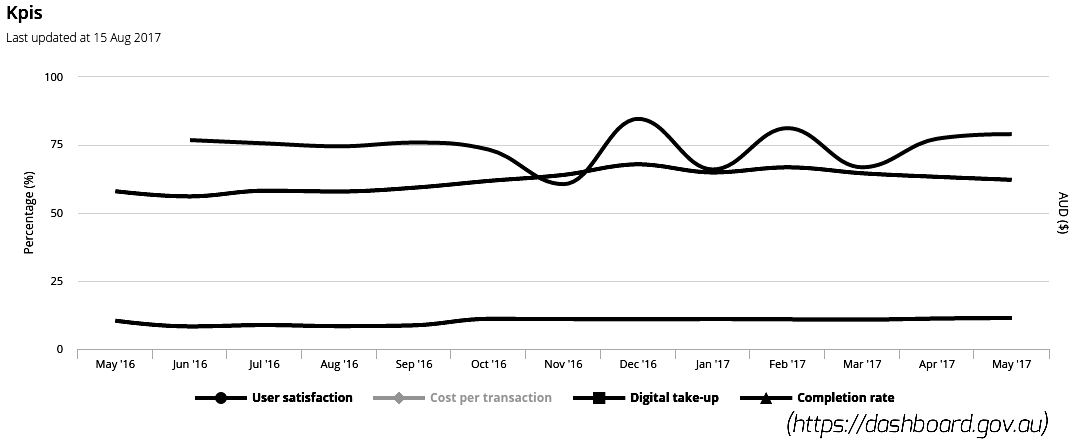
\includegraphics[width=0.99\textwidth]{kpis_dashboard_gov_au}
  \caption{KPIs del dashboard del gobierno de australia}
  \centering
  \label{fig:kpis_dashboard_gov_au} %\ref{fig:kpis_dashboard_gov_au}
  \end{figure}
  \FloatBarrier

En próximos capítulos vamos a ver irradiadores visuales que pueden servir como dashboard simples para uso bajo el marco Scrum.

\subsection{Métricas ágiles}

Por último, hay que tener en cuenta que para que las métricas estén bajo un marco Scrum deben respetar los principios de la agilidad. La medida principal es el software funcionando. Las métricas deben ser un medio de comunicación efectiva e impulsar la transparencia. Deben servir al equipo para que se auto-organize en procesos de corrección de desvíos y mejora contínua, apoyando la reflexión sobre cómo ser más efectivos. Y, principalmente, se debe buscar siempre la simplicidad. Las métricas que agregan complejidad innecesaria o sobre-información no son acordes a la agilidad. Lo difícil es encontrar el equilibrio entre un Scrum minimalista y hacer ingeniería. Si no medimos no podemos hacer análisis del sistema de trabajo, o sistema productivo, para mejorar con datos empíricos como lo requiere el trabajo ingenieril; pero si medimos excesivamente podemos estar generando desperdicio (burocracia y trabajo no relevante) y ruido informativo (datos que no generan información útil). Los KPI's no se deben convertir en objetivos que deben lograrse ni en herramienta de control de empleados.
